%======================================================================
\section{Study 1: first-order estimates against exact silencing}
\label{sec:study1}

All results in this section are from the \NConfModels{} confirmation models unless stated otherwise. All saved responses passed the checks described in \cref{app:verification}.

\subsection{The first-order estimate finds the cell types with large effects}
\label{sec:screening}

\Cref{tab:screen} compares the rankings at both strengths, and \cref{fig:screen} shows the precision of each model at full silencing. Of the ten cell types ranked highest by the first-order estimate, a mean fraction of \PrecFOFull{} (95\% interval \PrecFOCIFull{}) had large effects at full silencing, against \PrecAnatFull{} \PrecAnatCIFull{} for three-step anatomical path weights and \PrecRandomFull{} for a random ranking. The paired difference was \PrecDiffAnatFull{} \PrecDiffAnatCIFull{}; the first-order estimate was higher in \PrecWinsAnatFull{} models, equal in \PrecTiesAnatFull{} and lower in \PrecLossesAnatFull{} (\cref{tab:paired}). Its recall was \RecallFOFull{}, against \RecallAnatFull{} for anatomy. At half strength the margin was larger: \PrecFOHalf{} against \PrecAnatHalf{}, a difference of \PrecDiffAnatHalf{} \PrecDiffAnatCIHalf{}, with the first-order estimate higher in all \PrecWinsAnatHalf{} models.

\begin{figure}[t]
  \centering
  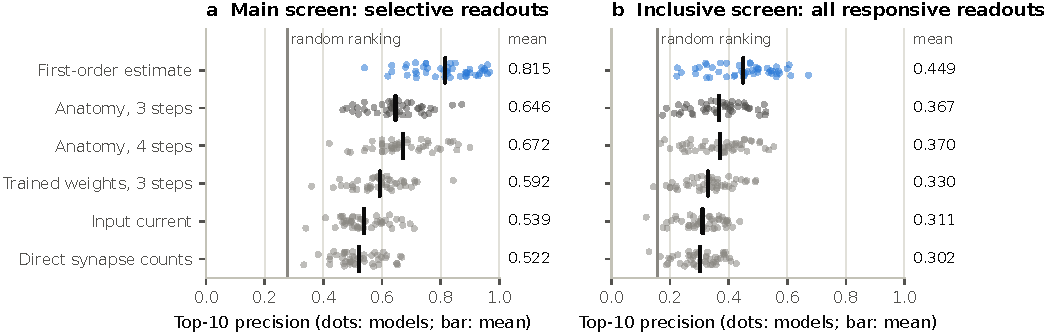
\includegraphics[width=\textwidth]{figures/s1-fig1-screening.pdf}
  \caption{Top-10 precision of each ranking at full silencing, one dot per confirmation model, with the mean as a bar and its value on the right. (a) Main screen: direction-selective readout conditions, large effect $|\Delta\DSI|\ge\LargeThreshold$. (b) Inclusive screen: all responsive readout conditions and all cell types, with abolished responses counted as large effects. The vertical line is the expected precision of a random ranking.}
  \label{fig:screen}
\end{figure}

\begin{table}[t]
  \centering
  \small
  \caption{Screening and ranking by each method, means over the \NConfModels{} confirmation models. Precision and recall refer to the ten highest-ranked cell types; Spearman $\rho$ compares each ranking with the magnitude of the exact change, over all scored cell types or over large effects only. The inclusive screen scores all responsive readout conditions and counts abolished responses as large effects. Bold: first-order estimate.}
  \label{tab:screen}
  \begin{tabular}{lcccccc}
    \toprule
    & \multicolumn{2}{c}{Top-10 precision} & Recall & \multicolumn{2}{c}{Spearman $\rho$, $s=1$} & Inclusive \\
    \cmidrule(lr){2-3}\cmidrule(lr){5-6}
    Ranking & $s=0.5$ & $s=1$ & $s=1$ & all & large & precision, $s=1$ \\
    \midrule
    \tableinput{generated/s1-table-screen.tex}
  \end{tabular}
\end{table}

Anatomical precision at full silencing rose with path length, from \PrecAnatOneFull{} for one step (the same ranking as direct synapse counts) to \PrecAnatTwoFull{}, \PrecAnatFull{} and \PrecAnatFourFull{} for two, three and four steps; graph distance reached \PrecDistFull{}. The four-step variant, the best of these, still trailed the first-order estimate by \PrecDiffAnatFourFull{} \PrecDiffAnatFourCIFull{}. Rankings that use the trained models fell below anatomy: trained-weight path weights reached \PrecTrainedFull{} and the intact input currents \PrecCurrentFull{}. Over all scored cell types, the first-order ranking agreed far more closely with the exact one than any other ranking (Spearman correlation \RhoFOFull{}, against \RhoAnatFull{} for three-step anatomy).

The inclusive screen gave \InclFOFull{} \InclFOCIFull{} for the first-order estimate and \InclAnatFull{} \InclAnatCIFull{} for three-step anatomy, against \InclRandomFull{} for a random ranking (\cref{fig:screen}b). Its precisions are lower for every method because the readout conditions with weak selectivity that it adds have few large changes: a random ranking would score \InclRandomLowDSIFull{} there and \InclRandomMainDSIFull{} in the direction-selective ones (post hoc). The paired difference was \InclDiffAnatFull{} \InclDiffAnatCIFull{}, computed post hoc with the prespecified bootstrap, and the first-order estimate was higher in \InclWinsAnatFull{} models, equal in \InclTiesAnatFull{} and lower in \InclLossesAnatFull{}.

\begin{table}[t]
  \centering
  \small
  \caption{Paired comparisons at full silencing: first-order estimate minus each ranking, means over models with 95\% bootstrap intervals, and the numbers of models in which the first-order value is higher, equal or lower (higher and lower for correlations). Correlation differences among large effects use the readout conditions in which both correlations exist (\RhoUnitsFull{} for three-step anatomy).}
  \label{tab:paired}
  \footnotesize
  \setlength{\tabcolsep}{4pt}
  \begin{tabular}{lcccc}
    \toprule
    & \multicolumn{2}{c}{Top-10 precision} & \multicolumn{2}{c}{Spearman $\rho$, large effects} \\
    \cmidrule(lr){2-3}\cmidrule(lr){4-5}
    Ranking & Difference [95\% interval] & Higher/equal/lower & Difference [95\% interval] & Higher/lower \\
    \midrule
    \tableinput{generated/s1-table-paired.tex}
  \end{tabular}
\end{table}

\subsection{The first-order estimate misjudges the size and sign of the effects}
\label{sec:effects}

\Cref{fig:s1-scatter} plots every scored case. At both strengths the estimates scatter widely around the line of equality. Pooled over cases (post hoc), the Pearson correlation between estimate and exact change was \PearsonPooledHalf{} at half strength and \PearsonPooledFull{} at full silencing; at full silencing, \LargeDecPredIncPct\% of the \LargeDecFull{} large decreases of selectivity were predicted as increases and \LargeIncPredDecPct\% of the \LargeIncFull{} large increases as decreases, and \AbsPredAboveOneFull{} estimates exceeded 1 in magnitude, a change larger than the whole range of the index allows (the largest was \MaxAbsPredFull{}).

\begin{figure}[t]
  \centering
  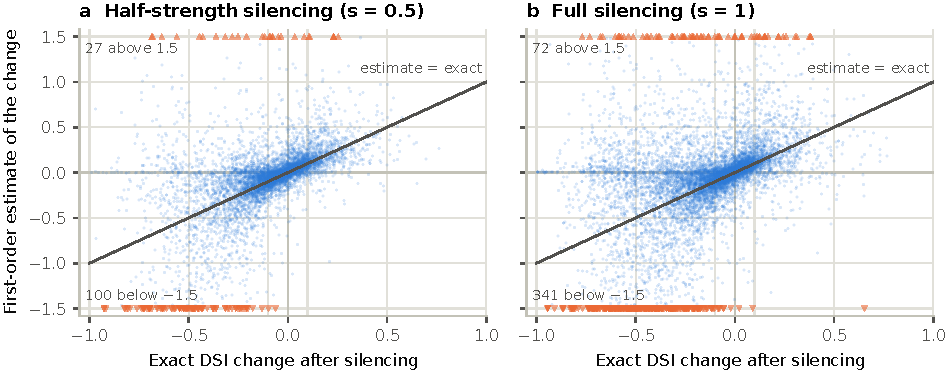
\includegraphics[width=\textwidth]{figures/s1-fig2-predicted-vs-exact.pdf}
  \caption{First-order estimate against exact change in DSI for every scored silencing case, pooled over the confirmation models: (a) \MainCasesHalf{} cases at half strength, (b) \MainCasesFull{} at full silencing. The diagonal marks equality and the grey vertical lines mark the large-effect threshold $|\Delta\DSI|=\LargeThreshold$. Estimates beyond the plotted range are drawn at its edge as triangles, with their numbers given in the panels.}
  \label{fig:s1-scatter}
\end{figure}

\Cref{tab:magnitude} gives the errors. At full silencing the mean absolute error of the first-order estimate was \MaeFOFull{} \MaeFOCIFull{}, and predicting zero change gave \MaeZeroFull{} \MaeZeroCIFull{}. The paired difference was \MaeDiffFull{} \MaeDiffCIFull{}, and the first-order error was the larger one in \MaeWorseFull{} of \NConfModels{} models (\cref{fig:errors}b; every model is listed in \cref{app:models}). The errors run in both directions: the mean signed error was \BiasFull{} \BiasCIFull{} (summarised post hoc), and it ranged from \BiasMinFull{} to \BiasMaxFull{} across models. Among the \LargeFull{} large changes (\LargeFullPct\% of scored cases) the first-order error was \MaeLargeFOFull{} against \MaeLargeZeroFull{} for zero change, and \WrongSignFull\% \WrongSignCIFull{} of the estimates had the wrong sign; the model with the fewest sign errors had \WrongSignMinFull\% and the one with the most \WrongSignMaxFull\%. Only \ZeroPredFull\% of large changes had an estimate of exactly zero, so the sign errors come from estimates pointing the wrong way rather than from missing ones.

\begin{table}[t]
  \centering
  \small
  \caption{Effect-size errors in the main analysis, means over the \NConfModels{} confirmation models with 95\% bootstrap intervals. Errors are pooled over each model's scored cases before averaging over models. The mean signed error is first-order estimate minus exact change (summarised post hoc).}
  \label{tab:magnitude}
  \begin{tabular}{lcc}
    \toprule
    & Half strength ($s=0.5$) & Full silencing ($s=1$) \\
    \midrule
    \tableinput{generated/s1-table-magnitude.tex}
  \end{tabular}
\end{table}

Clipping each estimate so that the predicted index stays in $[0,1]$ lowered the error to \MaeClipFull{}, below predicting zero change by \ClipDiffFull{} \ClipDiffCIFull{} and in \ClipBetterFull{} of \NConfModels{} models. Before clipping, \OutsideFull\% of the estimates placed the index outside its possible range. Clipping removes impossible values but leaves the wrong signs in place.

At half strength the first-order error, \MaeFOHalf{}, was close to the zero-change error, \MaeZeroHalf{} (difference \MaeDiffHalf{} \MaeDiffCIHalf{}); it was the larger error in \MaeWorseHalf{} models and the smaller in \MaeBetterHalf{}. Of the large changes, \WrongSignHalf\% had the wrong sign, and the clipped estimate reached \MaeClipHalf{}. When every responsive readout condition and every case with a defined DSI is included, the full-silencing errors were \InclMaeFOFull{} for the first-order estimate, \InclMaeZeroFull{} for zero change and \InclMaeClipFull{} for the clipped estimate (\cref{app:sensitivity}).

\begin{figure}[t]
  \centering
  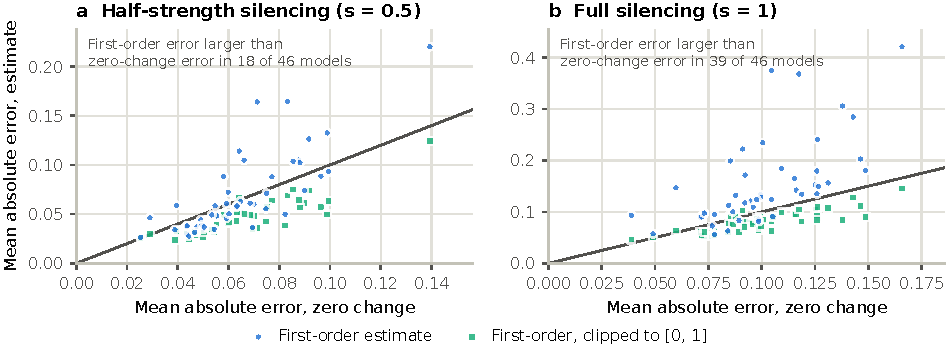
\includegraphics[width=\textwidth]{figures/s1-fig3-model-errors.pdf}
  \caption{Mean absolute error of the first-order estimate (circles) and of the clipped estimate (squares) against that of predicting zero change, one point per confirmation model: (a) half strength, (b) full silencing. Points above the diagonal are models in which the estimate is less accurate than predicting zero change.}
  \label{fig:errors}
\end{figure}

\subsection{Among large effects, the ranking is no better than anatomy}
\label{sec:ranking}

Separating large from small effects and ordering the large effects are different tasks. Among large effects only, the Spearman correlation of the first-order ranking with the exact change at full silencing was \RhoLargeFOFull{}, against \RhoLargeAnatFull{} for three-step anatomy and \RhoLargeTrainedFull{} for trained-weight path weights (\cref{tab:screen}). The paired difference from anatomy was \RhoLargeDiffAnatFull{} \RhoLargeDiffAnatCIFull{}, and the first-order estimate was higher in \RhoLargeWinsAnatFull{} of \RhoLargeModelsAnatFull{} models (\cref{tab:paired}). At half strength it ranked large effects better than anatomy (\RhoLargeFOHalf{} against \RhoLargeAnatHalf{}, difference \RhoLargeDiffAnatHalf{} \RhoLargeDiffAnatCIHalf{}; higher in \RhoLargeWinsAnatHalf{} models). Its advantage at full silencing is therefore in separating large effects from small ones.

\subsection{The error grows with silencing strength}
\label{sec:s1-strength}

The development models were also silenced at strengths 0.1, 0.25 and 0.75 (\cref{fig:s1-strength}; \cref{app:development}). The first-order error grew faster with strength than the zero-change error: it was the smaller of the two at strength 0.1 (\DevMaeFOOneTenth{} against \DevMaeZeroOneTenth{}) and 0.25 (\DevMaeFOQuarter{} against \DevMaeZeroQuarter{}) and the larger from 0.5 on, reaching \DevMaeFOFull{} against \DevMaeZeroFull{} at full silencing. It was the more accurate predictor in every development model at strength 0.1, in \DevBetterQuarter{} of \NDevModels{} at 0.25 and in none at 0.75 or 1. Screening precision rose with strength for both rankings because more changes exceed the fixed threshold, and the first-order estimate led anatomy at every strength (\DevPrecFOOneTenth{} against \DevPrecAnatOneTenth{} at 0.1, \DevPrecFOFull{} against \DevPrecAnatFull{} at 1). At full and half strength the development models agree with the confirmation results.

\begin{figure}[t]
  \centering
  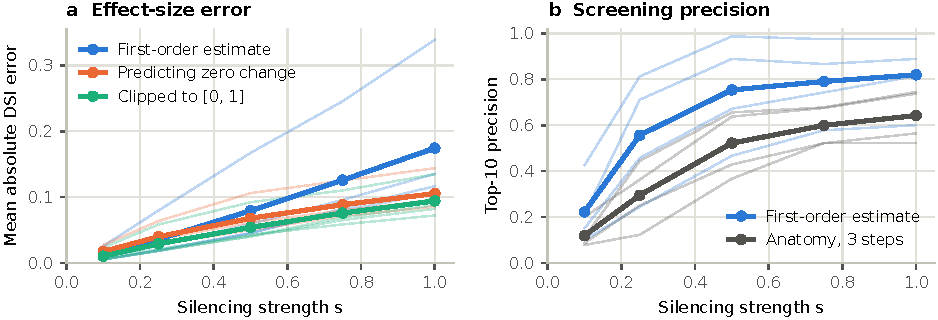
\includegraphics[width=\textwidth]{figures/s1-fig4-strength.pdf}
  \caption{Dependence on silencing strength in the four development models. (a) Mean absolute error of the first-order estimate, of predicting zero change and of the clipped estimate. (b) Top-10 precision of the first-order estimate and of three-step anatomy. Thin lines: individual models; thick lines: means. Each strength is scored on its own set of cases.}
  \label{fig:s1-strength}
\end{figure}

\subsection{Where the errors arise}
\label{sec:diagnostics}

The errors are concentrated in a minority of cases (\cref{tab:diagnostics}). For changes smaller than \LargeThreshold{} the median absolute error was \MedianErrSmallFull{}, and for large changes \MedianErrLargeFull{}. Errors were larger when the silenced type synapses directly onto the readout cell (\MaeDirectFull{}, \InputDirectCases{} cases) than when it acts only through other cells (\MaeIndirectFull{}, \InputIndirectCases{} cases). They were largest when silencing changed the set of directions that evoke no response at all, by silencing a response or by creating one (\MaeZeroPeakChangedFull{} in \ZeroPeakChangedCases{} cases, against \MaeZeroPeakSameFull{} in \ZeroPeakSameCases{} cases where that set stayed the same). The derivative is blind to such changes: a direction with a zero peak contributes zero derivative, so a response that appears is missed, and a response that disappears is extrapolated linearly past the floor of zero. In readout conditions with intact DSI below \MainDSI{}, which the main analysis leaves out, the first-order error was \MaeLowDSIFull{} against \MaeZeroLowDSIFull{} for zero change over \LowDSICasesFull{} cases. These categories overlap and describe associations; Study 2 (\cref{sec:study2}) tests where the nonlinearity lies.

\begin{table}[t]
  \centering
  \small
  \caption{Errors at full silencing by kind of case. Left: the main analysis, with the share of first-order estimates that place the index outside $[0,1]$. Right: all responsive readout conditions with a defined DSI after silencing, including amplified cases. Means over models of per-model mean absolute errors.}
  \label{tab:diagnostics}
  \footnotesize
  \setlength{\tabcolsep}{4.5pt}
  \begin{tabular}{lrcccrcc}
    \toprule
    & \multicolumn{4}{c}{Main analysis} & \multicolumn{3}{c}{All responsive} \\
    \cmidrule(lr){2-5}\cmidrule(lr){6-8}
    Cases & Number & First-order & Zero & Outside (\%) & Number & First-order & Zero \\
    \midrule
    \tableinput{generated/s1-table-diagnostics.tex}
  \end{tabular}
\end{table}

\subsection{Abolished, unchanged and amplified responses}
\label{sec:abolition}

Full silencing abolished the response of the readout in \AbolishedFull{} of the \ResponsiveCases{} cases in responsive readout conditions (\AbolishedFullPct\%), spread over \AbolitionReadoutsFull{} readout conditions; half strength abolished \AbolishedHalf{}. Silencing Mi1 caused \AbolishedByMiOne{} abolitions, L1 \AbolishedByLOne{}, Mi4 \AbolishedByMiFour{} and Tm3 \AbolishedByTmThree{} (post hoc counts). Where the response survived, its amplitude usually changed little: the median ratio of preferred-polarity peak responses after and before full silencing was \AmpRatioMedian{} (quartiles \AmpRatioQOne{} and \AmpRatioQThree{}; 5th and 95th percentiles \AmpRatioLowQ{} and \AmpRatioHighQ{}), with \AmpRatioBelowHalfPct\% of ratios below one half and \AmpRatioAboveTwoPct\% above two (post hoc). Large changes of selectivity came with larger changes of amplitude (median ratio \AmpRatioLargeMedian{}, quartiles \AmpRatioLargeQOne{} and \AmpRatioLargeQThree{}): large decreases of selectivity typically came with larger responses (median \AmpRatioLargeDecMedian{}) and large increases with smaller ones (median \AmpRatioLargeIncMedian{}; post hoc).

In \ZeroGradReadouts{} readout conditions every first-order estimate was exactly zero. Of these, \Unresponsive{} have no response at all, and in \ZeroGradResponsiveSilent{} the readout responds only to edges of the other polarity, so its DSI is 0 and its rectified peaks give zero derivative. In the remaining \ZeroGradSelective{}, all in the main analysis, a single direction of the preferred polarity evokes a response, so the DSI equals 1 whatever the size of that response; full silencing nevertheless abolished the response for \ZeroGradAbolitionsRange{} cell types in each of them (post hoc).

Amplification beyond \AmpLimit{} times the largest intact readout voltage followed \AmplifiedInterventionsFull{} full-silencing interventions (each a model, stimulus and cell type), affecting \AmplifiedCasesFull{} responsive cases, and \AmplifiedInterventionsHalf{} interventions at half strength (\AmplifiedCasesHalf{} cases); \cref{app:coverage} counts all exclusions.

\subsection{Thresholds, tuning groups and pairs}
\label{sec:robustness}

The comparison holds across the prespecified thresholds (\cref{app:sensitivity}). For the \SensCombos{} combinations of a DSI threshold of at least 0.1 with an amplification limit of \AmpLimitLow{}, \AmpLimit{}, \AmpLimitHigh{} or none, first-order precision at full silencing ranged from \SensPrecFOMin{} to \SensPrecFOMax{} and anatomical precision from \SensPrecAnatMin{} to \SensPrecAnatMax{}, and in all \SensCombosAll{} combinations, including a DSI threshold of 0, the first-order error exceeded the zero-change error. The three groups of models with upward, downward and weak T4c tuning~\citep{lappalainen2024connectome} gave the same picture (\cref{app:clusters}): first-order precision was \ClusterUpPrec{}, \ClusterDownPrec{} and \ClusterWeakPrec{}, and at full silencing the first-order error exceeded the zero-change error in each group. In the development models, silencing two input types of T4 together often changed the DSI by more or less than the sum of the single effects (median absolute interaction \PairMiOneMiFourDSI{} for Mi1 with Mi4), while pairs of T5 inputs interacted weakly (\cref{app:pairs}).
